\documentclass[a4paper, 12pt]{report}
\usepackage{graphicx}
\begin{document}

\title{Smarter and simple Scrabble strategy}
\date{Course: DD143X \\ Supervisor: Johan Boye \\ Kungliga Tekniska Högskolan \\ CSC \\ March 7, 2012}
\author{Frej Connolly \\ Götgatan 78 13TR LÄG1302 \\ 118 30 Stockholm \\ SWEDEN \\ +46(0)73-963 41 90 \\ connolly@kth.se \\
        \and Diana Gren \\ Sköldgatan 8 2TR \\ 118 63 Stockholm \\ SWEDEN \\ +46(0)70-467 47 20 \\ dianagr@kth.se}

\maketitle
\tableofcontents


\chapter{Introduction}
Scrabble is an old classic word game that requires a great pool of knowledge and a sharp eye from the players. It was invented in the early 90s, and was first sold in 1949 \cite{scrabbleforbund}. Ever since the computer started to take place, there has been attempts to create an agent that would play Scrabble and win. The first one is called \emph{Maven} and is even today a very powerful player.

Wordfeud is an immensely popular software implementation for smart phones. The most significant difference to Scrabble is that it is restricted to be played by only two players.

\section{Game rules}
Two or four players form words to lay down on a 15 by 15 grid game board. Words can be placed across or downwards. Each word has to be placed adjacent to a word (except the first round) and must appear in a standard dictionary. Each tile contains one letter, which give different points depending on how common they are in the language.  

Some squares on the game board contain bonuses, that will either double or triple the point of the letter placed on it, or double or triple the score of the whole word placed. If all tiles on hand are placed on the game word an additional 50 points are rewarded. The game ends when one player have placed out all their tiles on the game board and there’s no tiles left to pick up. At that point, the score is calculated and the player with the highest score wins.

\section{Problem statement}
The game require the players to have a good vocabulary and keeping an extra eye on which letter tiles that have already been placed and those who award the most points. Keeping a good balance between consonant and vocals on hand is a key to able to master the next move. It’s important to score bonus and prevent to opponent doing the same, by avoiding placing tiles that opens up a bonus square.

This gives the player many factors to take in consideration every time a move is to be made. Such factors are; words that generate higher scores, bonus tiles etc.

If there were to be a strategy where only one of these factors would be considered, which one would be the most rewarding? This study aims to investigate which of these factors has the bigger impact when one is reaching for a win. Three different programmed agents with three different objectives will play against each other in order to show results and let us determine the most preferable strategy.


\chapter{Background}
How to play a close to perfect game of Scrabble is a well studied problem. It is not as trivial as chess, checkers or tic tac toe, since there are many factors included in Scrabble that are not a part of the other classical games. For further explanations we shall introduce the expressions \emph{deterministic} and \emph{non-deterministic}. 

\begin{description}
\item[Deterministic] A game is deterministic if the players have all possible information about the state of the game, and possible future states.
\item[Non-deterministic] In contrast to a deterministic game, a non-deterministic game does not let the players now all information about the game's current or future states.
\end{description}

Unfortunately, it is not as easy to determine in which folder to put the game of Scrabble. It is not a deterministic game for sure, since we do not know which tiles are possessed by the opponent. At the same time, one could not say that it is completely non-deterministic. Imagine the end of a game, at that time all the tiles are either on the board, on the player's hand or on the opponent's hand. This results in a situation where one could figure out the complete information scope of the current state. Of course, this requires the player to know exactly how many pieces of each tiles exist in the game.

\chapter{Analysis}
This chapter will describe solutions of one of the major problems when implementing the agent; the dictionary representation. Which solution that in the end was chosen, and why, will also be explained. The considered game strategies to investigate are presented in the second section of the chapter.

\section{Dictionary representation}
When playing Scrabble in a tournament each player needs to finish all the rounds within a time frame, usually 25 minutes. Which means searching for words needs to be fast. The dictionary can be represented i several different waysand studies have been made in which is the most efficient strategy in both memory space and time cost, with the result being GADDAG and DAWG \cite{faster}\cite{fastest}, both different tyoes of minimizations of a trie. This section will look deeper into each of the alternatives, and explain both advantages and disadvantages with each of them.

This study used a Trie, with the reason that it would be fairly easy to implement, but still be a powerful tool when searching for words. The words included are from the Swedish Dictionary, witch is available online for download. All words are represented on the normal form to simplify and keep the study within reasonable limits. This resulted in a dicitonary consisting of a little over 52000 words.

\subsection{Trie}

\begin{figure}
\centering
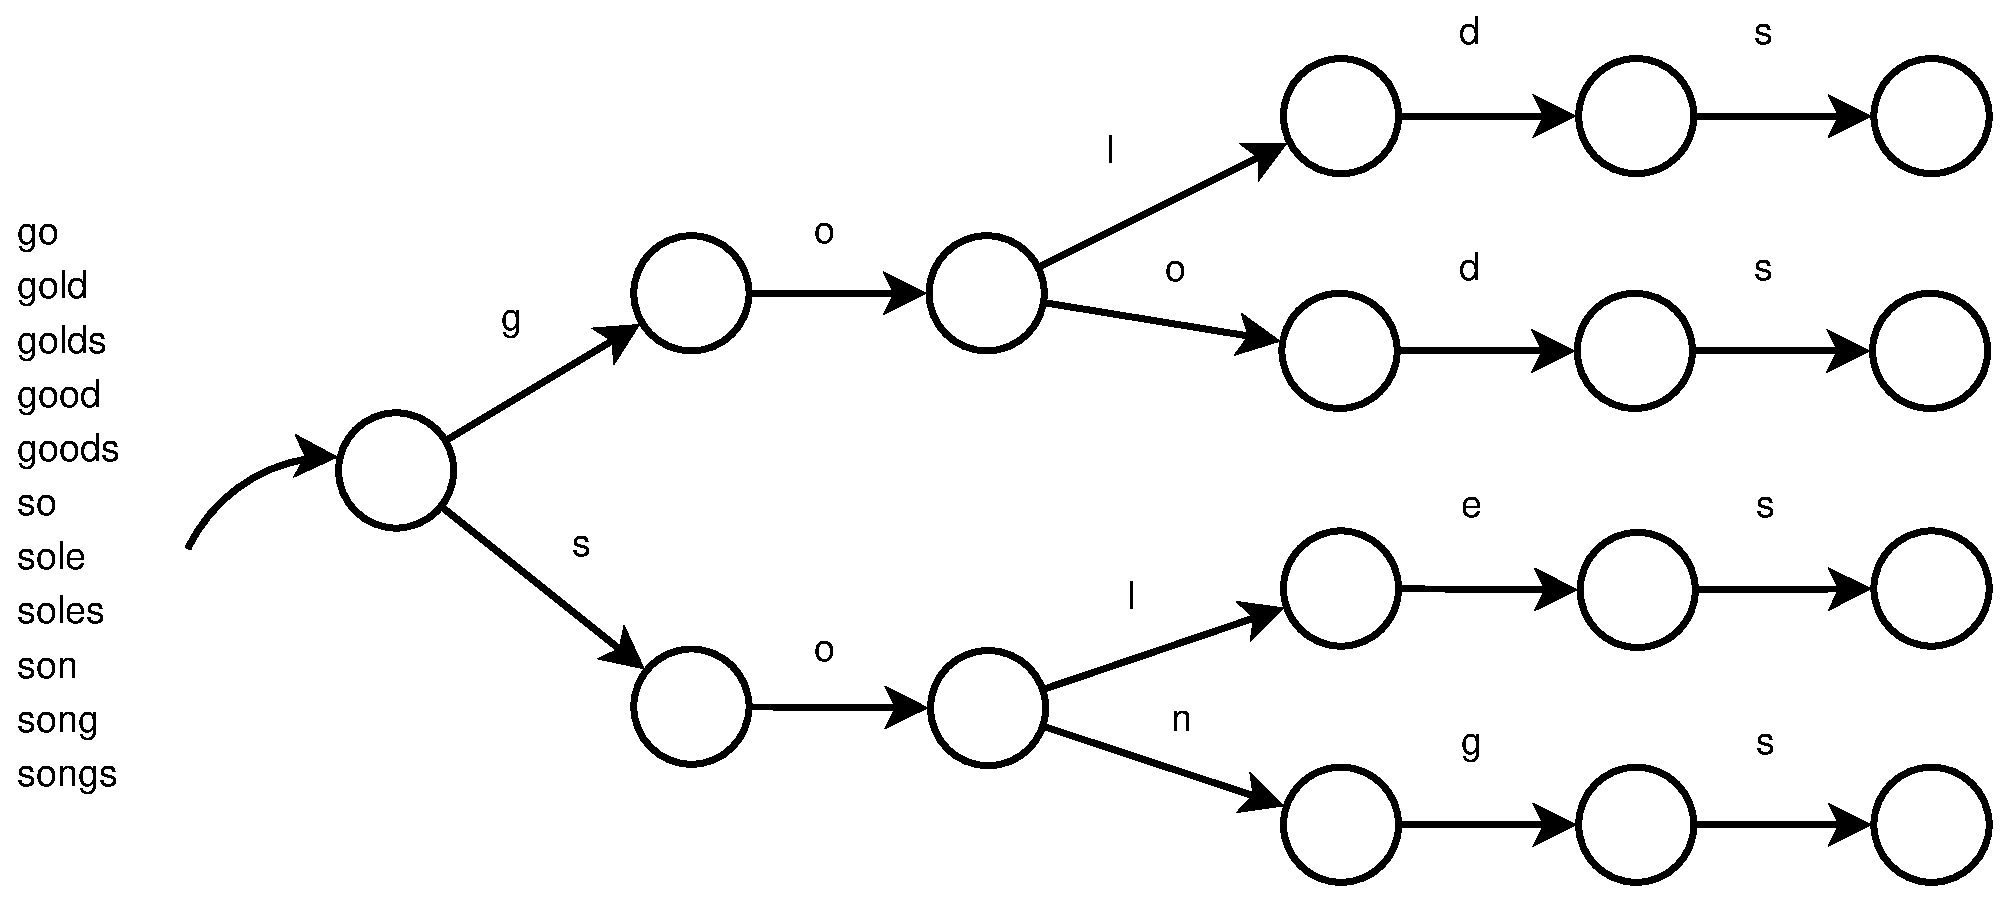
\includegraphics[scale=0.6]{trie}
\caption{Words represented as a Trie}
\end{figure}
\subsection{DAWG}
Appel and Jacobson \cite{fastest} showed that when using a directed acyclic word graph DAWG it's easy to find legit words. The data structure is an evolution of a trie where each word corresponds to a path from the root. Each edge representing a letter and nodes flags end of a word. At the time discovering the DAWG disk space were limited and an English dictionary with 94240 words would take up 117150 nodes and 179618 edges. It would occupy over half a megabyte.

By using a directed graph instead and letting nodes be shared by several edges it would dramatically reduce size to 19853 nodes and disk space 175 kB. For example the words awesome, awesomeness, awesomely would all share the first 7 nodes. When adding the word greatly it could share the last two letters l and y with the same nodes as the last two for awesomely. Nodes mark the the end of words with a boolean EOW.

\subsection{GADDAG}
\section{Game strategies}
This study will focus on investigating three types of strategies, where all three will have one main objective each to take in consideration:
\begin{description}
\item[High score words] The agent will search through possible words to place, and choose the one where the word only gives the highest score.
\item[Bonus squares] Instead of focusing on the word, this agent will try to reach the bonus squares at all times.
\item[Balance on hand] To avoid deadlocks (i.e. a situation where no move can be made) the agent will try to keep a good balance between vowels and consonants on hand. 
\end{description}
\subsection{High score words}
One approach in the game of Scrabble, is to try to lay out the words that will generate the highest score without considering other factors, such as bonus squares. This means, that the word either has to be very long, or use letters with high score points. Another idea is also that many words are created with one move, which, of course, can only be accomplished after the first move has been made.
\subsection{Bonus squares}
\subsection{Balance on hand}
\chapter{Results}
\chapter{Conclusions}
\chapter{Discussion}


\begin{thebibliography}{100}  
  \bibitem{perfectgame} Sheppard, B., 2002, Towards Perfect Play of Scrabble, Maastricht.
  \bibitem{fastest} Appel A. W., Jacobson, G. J., 1985, The World’s Fastest Scrabble Program, Commun. ACM, 31(5), 572-585, May 1988.
\bibitem{faster} Gordon, S. A., 1993, A Faster Scrabble Move Generation Algorithm, Software - Practice and experience, Vol. 24(2), 219-232, February 1994.
\bibitem{quakle} Katz-Brown, J., O’Laughlin, J., Fultz, J., Liberty, M., Buddhdev, A., 2006, Quakle - open source crossword game software, http://people.csail.mit.edu/jasonkb/quackle/, 2 January 2012,  12 February 2012.
\bibitem{scrabblewiki} Wikipedia, Scrabble, http://en.wikipedia.org/wiki/Scrabble, 12 February 2012.
\bibitem{frank} Andersson, G., Ivansson, L., Frank - crossword software game, http://ivansson.org/Frank/, 22 August 2009, 12 February 2012.
\bibitem{wordfeud} Hbwares, Wordfeud, http://www.wordfeud.com, September 2010, 12 February 2012.
\bibitem{ai} Russell S., Norvig P. Artificial Intelligence: A Modern Approach 3rd ed. Prentice Hall. 2009
\bibitem{inforetrieve} Manning C. D., Raghavan P., Schütze H., Introduction to Information Retrieval, Cambridge University Press, 2008, p. 49-65.
\bibitem{scrabbleforbund} Svenska Scrabbleförbundet, www.scrabbleforbundet.se.
\end{thebibliography}
\end{document}
